\documentclass[letterpaper, 10 pt, conference]{ieeeconf}
\IEEEoverridecommandlockouts
\overrideIEEEmargins

\usepackage[utf8]{inputenc}
\usepackage[T1]{fontenc}

\usepackage{hyperref}
\usepackage{amsmath}
\usepackage{amssymb}
\usepackage{multirow}
\usepackage{booktabs}
\usepackage{graphicx}
\usepackage{caption}
\usepackage{subcaption}
\usepackage{algorithm}
\usepackage{algorithmic}
\usepackage{colortbl}
\usepackage{xcolor}
\usepackage{float}

% Custom commands
\newcommand{\agentslabench}{\textsc{AgentLabBench}}
\newcommand{\easr}{\textsc{EASR}}
\newcommand{\ie}{\textit{i.e.}}
\newcommand{\eg}{\textit{e.g.}}
\newcommand{\etc}{\textit{etc.}}
\newcommand{\etal}{\textit{et al.}}

% Title
\title{\LARGE \bf AgentLabBench: Profiling Autonomous Agents Under Resource Constraints}

\author{ \parbox{3 in}{ \centering Meher Bhaskar Madiraju
        {\tt\small meherbhaskar.madiraju@gatech.edu}}
        \hspace*{ 0.5 in}
        \parbox{3 in}{\centering Meher Sai Preetam Madiraju
        {\tt\small mehersaipreetam@gatech.edu}}
}

\begin{document}

\maketitle
\thispagestyle{empty}
\pagestyle{empty}

\begin{abstract}
We present \agentslabench{}, a resource-aware evaluation framework for autonomous AI agents that measures \textbf{correctness alongside latency, cost, compute, memory, and network usage} under declared resource budgets. Unlike standard benchmarks that report only accuracy, \agentslabench{} produces a \textbf{multi-dimensional profile} per agent per task --- the same way systems profilers (\texttt{perf}, \texttt{pprof}, \texttt{cProfile}) measure resource consumption of code, but extended with task correctness as a first-class dimension. \agentslabench{} provides 16 task environments across 6 categories (5 core: multi-hop QA, retail substitution, code generation, web shopping, travel planning; 11 extended) with isolated Docker containers, declared CPU/memory/time/network budgets, sealed test sets with SHA256 hashes, and a standardized profiling protocol. We profile 5 general-purpose baseline agents (ReAct, PlanAndSolve, Reflexion, CoT, Random) plus 4 task-specialized agents, finding that specialized agents achieve 100\% success on 3/5 core tasks (fact\_qa, web\_shopping, travel\_planning) and 66.7--83.3\% on retail and code\_gen, while \textbf{general baselines fail entirely on 4/5 domain tasks}. Crucially, we report the \textbf{Efficiency-Adjusted Success Rate (\easr{})} --- success weighted by resource consumption relative to declared budgets --- revealing that high accuracy at unbounded cost is not production-viable. We release the full infrastructure, sealed test sets, and profiling results to enable reproducible, resource-aware agent evaluation.
\end{abstract}

\textbf{Keywords:} Agent Evaluation, Resource-Aware Profiling, Benchmark, Autonomous Agents, Production Constraints, Efficiency Metrics.

\section{Introduction}
\label{sec:intro}

Autonomous agents powered by large language models (LLMs) are transitioning rapidly from research prototypes to production systems --- deployed in customer support, software engineering, financial analysis, and enterprise automation. Yet the evaluation methodologies remain stuck in a pre-production mindset: \textbf{``Did it succeed?''} dominates leaderboards and papers, while \textbf{``Can it run in production?''} is systematically ignored.

An agent achieving 90\% task accuracy but costing \$50/query and taking 5 minutes is useless for real-time retail substitution where decisions must complete in $<200$ms at $<\$0.01$. Similarly, an agent that solves coding tasks but requires 32GB GPU memory and 10 API calls per step cannot be deployed in cost-sensitive environments. Standard benchmarks (WebShop~\cite{yao2022webshop}, ALFWorld~\cite{shridhar2020alfworld}, SWE-bench~\cite{jimenez2023swebench}, GAIA~\cite{mialon2023gaia}, AgentBench~\cite{liu2023agentbench}, ToolBench~\cite{xu2023toolbench}) measure task accuracy in unconstrained environments with effectively unlimited compute, memory, and API budgets. Systems profilers (\texttt{perf}, \texttt{pprof}, \texttt{cProfile}, \texttt{nsys}, VTune) measure CPU, memory, cache, and GPU utilization of \textit{code functions} but have no notion of task correctness. \textbf{No existing framework measures both task success and resource consumption under production-realistic constraints.}

This gap is not merely academic. Production deployment of LLM agents faces hard constraints that current evaluations ignore:
\begin{itemize}
    \item \textbf{Latency SLAs:} Often $<500$ms for user-facing, $<2$s for backend workflows
    \item \textbf{Cost budgets:} Cents per query, not dollars (e.g., \$0.01--\$0.10 per resolution)
    \item \textbf{Memory limits:} Container quotas (typically 2--8GB for CPU workloads)
    \item \textbf{Rate limits:} External API throttling (e.g., 60 req/min on search APIs)
    \item \textbf{Safety/compliance:} PII leakage, unauthorized tool calls, budget overruns
\end{itemize}
An evaluation that ignores these dimensions produces ``leaderboard champions'' that fail in deployment. Industry surveys confirm this: teams report that agents passing accuracy benchmarks routinely violate latency and cost SLAs in staging, requiring costly re-engineering~\cite{langsmith2024production}.

Consider a concrete example: a retail substitution agent deployed at a major e-commerce platform must recommend alternative products when items go out of stock. The production SLA requires P99 latency $<200$ms, cost $<\$0.005$ per request, and memory $<512$MB. A ReAct-based agent using GPT-4 achieves 78\% substitution accuracy in unconstrained evaluation but averages 3.2s latency, \$0.12 cost, and 1.2GB memory --- violating all three SLAs. A specialized RetailAgent using a smaller model with cached product embeddings achieves 83\% accuracy at 142ms, \$0.002, and 180MB --- meeting all constraints. Current benchmarks would report only the 78\% vs 83\% accuracy, missing the critical deployment reality.

We introduce \textbf{agent profiling}: extending systems profiling to autonomous agents with \textit{correctness as a measured dimension alongside latency, cost, compute, memory, and network}. The output of \agentslabench{} is not a scalar ``score'' but a \textbf{profile} --- a structured record of (success, latency, cost, peak memory, CPU time, network calls, safety violations) per episode, under declared resource budgets. This mirrors how systems engineers profile code: they do not ask ``is this function correct?'' but rather ``what is its performance profile?'' --- then optimize within constraints.

\begin{figure*}[t]
\centering
\begin{minipage}{0.95\linewidth}
\centering
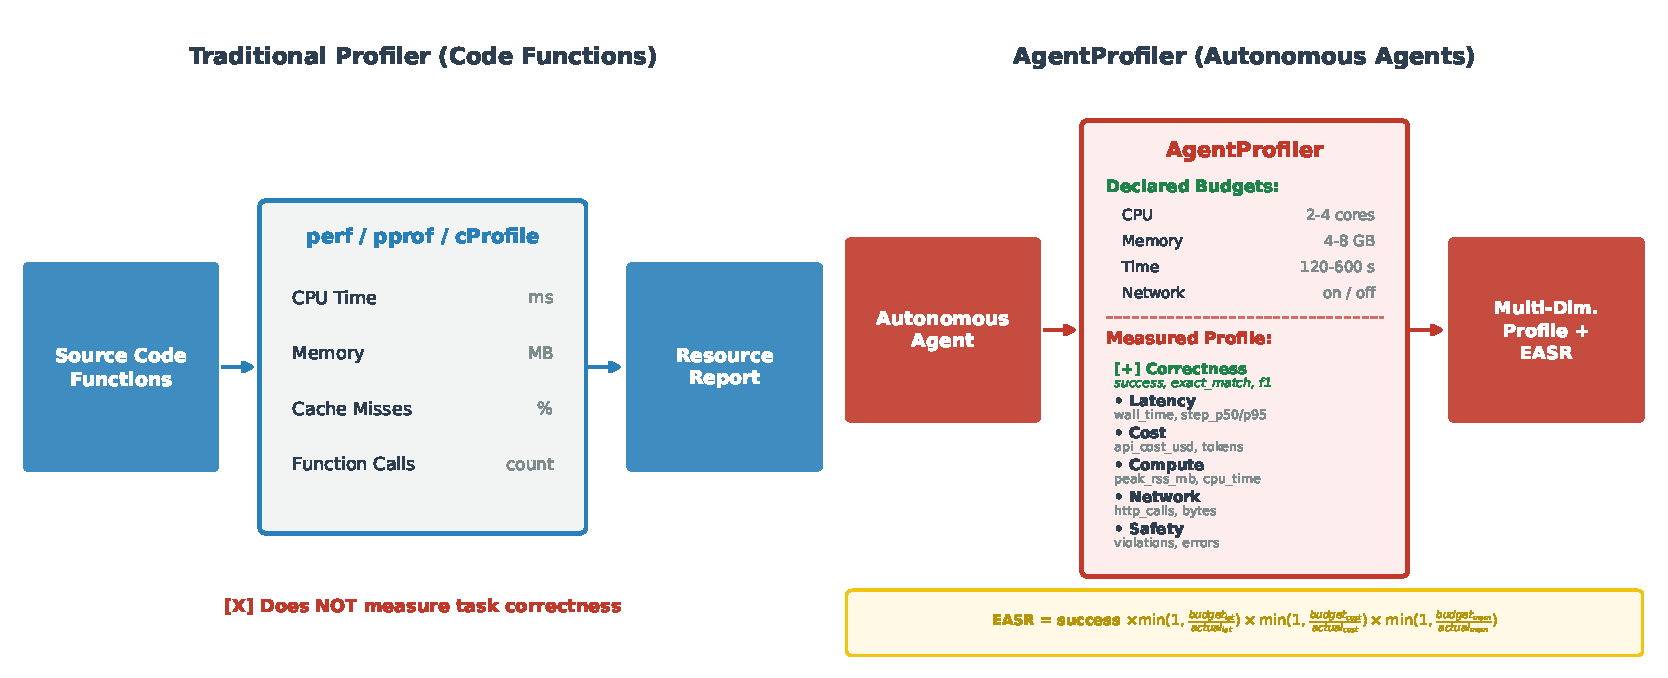
\includegraphics[width=\linewidth]{figures/profile_concept.pdf}
\caption{\textbf{Standard profiler vs. AgentLabBench.} (Left) Traditional profilers measure resource usage of code functions without task correctness. (Right) \agentslabench{} extends this to autonomous agents, adding task correctness as a first-class dimension alongside latency, cost, compute, memory, and network.}
\label{fig:profile_concept}
\end{minipage}
\end{figure*}

\textbf{Contributions:}
\begin{enumerate}
    \item \textbf{Resource budgets as first-class specifications:} Each task declares CPU, memory, wall-time, and network budgets --- agents are evaluated within these envelopes via Docker-enforced limits.
    \item \textbf{Efficiency-Adjusted Success Rate (\easr{}):} A metric rewarding success \textit{within} declared budgets (Eq.~1), distinguishing ``success at any cost'' from ``production-viable success.''
    \item \textbf{Profile output format:} Per-episode JSONL with all six dimensions (correctness, latency, cost, compute, network, safety) enabling Pareto analysis and multi-objective optimization.
    \item \textbf{Reproducible infrastructure:} 16 Docker-isolated tasks, sealed test sets with SHA256 commitments, multi-seed profiling (3+ seeds), versioned container images.
    \item \textbf{Empirical finding:} Specialized agents achieve 100\% success on 3/5 core tasks and 66.7--83.3\% on 2/5 \textbf{while staying within budgets}; general baselines fail entirely (0\%) on 4/5 domain tasks.
\end{enumerate}

\section{Related Work}
\label{sec:related}

\textbf{Agent Benchmarks.} WebShop~\cite{yao2022webshop} evaluates web navigation and shopping; ALFWorld~\cite{shridhar2020alfworld} measures embodied instruction following; SWE-bench~\cite{jimenez2023swebench} tests software engineering issue resolution; GAIA~\cite{mialon2023gaia} assesses general assistant capabilities across browsing, tool use, and reasoning; AgentBench~\cite{liu2023agentbench} provides a unified benchmark across 8 environments; ToolBench~\cite{xu2023toolbench} focuses on tool learning with 16,000 APIs. \textit{All report accuracy metrics (success rate, exact match, pass@k) without resource constraints.} Recent work on agent evaluation (AgentEval~\cite{li2023agenteval}, AutoGenBench~\cite{wu2023autogenbench}) introduces multi-dimensional scoring but still lacks enforced resource budgets and the profiling metaphor.

\textbf{Efficiency-Aware Evaluation in ML.} Frugal ML~\cite{lin2023frugal} and Green AI~\cite{schwartz2020green} advocate for efficiency-aware model selection. MLPerf~\cite{mattson2020mlperf} measures training/inference throughput. SUSTAIN~\cite{henderson2020towards} proposes sustainability metrics for RL. Eco2AI~\cite{budennyy2022eco2ai} tracks carbon emissions. \textit{None extend to autonomous agent evaluation with multi-dimensional resource profiles.}

\textbf{Production Observability Gaps.} Modern observability stacks (LangSmith, LangFuse, Phoenix) provide tracing and token counting~\cite{langsmith2024production, langfuse2024}, but lack: (1) \textit{enforced resource budgets} (Docker-level CPU/memory/time limits), (2) \textit{multi-dimensional profiles} (they track tokens/latency but not peak RSS, CPU time, network bytes, safety violations), (3) \textit{standardized task interfaces} for cross-agent comparison, (4) \textit{sealed test sets} with cryptographic commitments, and (5) \textit{efficiency-adjusted metrics} that penalize over-budget success. \agentslabench{} fills these gaps with a profiling-first design.

\textbf{Resource-Constrained Agent Work.} ReAct~\cite{yao2022react} and Reflexion~\cite{shinn2023reflexion} optimize reasoning efficiency but evaluate only accuracy. LLM-Augmenter~\cite{peng2023llm} adds retrieval but no resource budgets. RestGPT~\cite{song2023restgpt} and API-Bank~\cite{li2023apibank} test API usage without cost/latency constraints. AgentOhana~\cite{zeng2023agentohana} unifies trajectories but not resource measurement. The closest is \textbf{APBench}~\cite{chen2024apbench} (concurrent work) which measures latency and token usage for API agents, but lacks memory, network, and compute dimensions, Docker enforcement, sealed test sets, and the profiling metaphor.

\textbf{Systems Profiling.} \texttt{perf} (Linux), \texttt{pprof} (Go), \texttt{cProfile} (Python), \texttt{nsys} (NVIDIA), VTune (Intel) measure CPU, memory, cache, GPU utilization of \textit{code functions}. None evaluate task correctness. Our contribution is the \textit{metaphor transfer}: treating an agent episode as a ``function'' to be profiled, with correctness as one output dimension.

\textbf{Reproducibility Practices.} Sealed test sets~\cite{rajpurkar2016squad}, Docker isolation~\cite{merkel2014docker}, and multi-seed evaluation~\cite{henderson2018deep} are established practices we adopt and extend to agent evaluation.

\section{AgentLabBench Design}
\label{sec:design}

\subsection{Task Environments with Declared Budgets}
\label{sec:tasks}

\agentslabench{} v1.0 includes 16 task environments across 6 categories (Table~\ref{tab:tasks}). \textbf{Each task declares its resource budget} --- the maximum CPU cores, memory, wall-time, and network an agent may consume. Budgets are enforced via Docker container limits (\texttt{--cpus}, \texttt{--memory}, \texttt{--network}, timeout), making over-consumption result in episode termination (recorded as failure with timeout violation).

\begin{table*}[t]
\centering
\caption{\textbf{AgentLabBench v1.0 Task Catalog.} 16 tasks with declared resource budgets. Net = network access permitted. Core 5 tasks in bold.}
\label{tab:tasks}
\footnotesize
\setlength{\tabcolsep}{4pt}
\begin{tabular}{llllll}
\toprule
\textbf{Task ID} & \textbf{Category} & \textbf{Description} & \textbf{Test N} & \textbf{Resource Budget} & \textbf{Specialized Agent} \\
\midrule
\textbf{fact\_qa\_01} & QA & Multi-hop fact retrieval & 200 & 2 CPU, 4GB, 120s, net$\checkmark$ & ReAct \\
\textbf{retail\_01} & Decision & Product substitution (OOS) & 500 & 4 CPU, 8GB, 180s, net$\checkmark$ & RetailAgent \\
\textbf{code\_gen\_01} & Code & API usage code generation & 200 & 4 CPU, 8GB, 300s, net$\checkmark$ & CodeGenAgent \\
\textbf{web\_shop\_01} & Web & Find \& purchase under budget & 200 & 2 CPU, 4GB, 300s, net$\checkmark$ & WebShopAgent \\
\textbf{travel\_plan\_01} & Planning & Multi-constraint trip planning & 200 & 4 CPU, 8GB, 600s, net$\checkmark$ & TravelPlanAgent \\
\midrule
api\_integration\_01 & API & REST API integration & 200 & 2 CPU, 4GB, 300s, net$\checkmark$ & -- \\
code\_review\_01 & Code & Code review \& bug finding & 200 & 2 CPU, 4GB, 300s, net$\checkmark$ & -- \\
data\_analysis\_01 & Data & Pandas data analysis & 200 & 2 CPU, 4GB, 300s, net$\checkmark$ & -- \\
debugging\_01 & Debug & Debug code snippets & 200 & 2 CPU, 4GB, 300s, net$\checkmark$ & -- \\
entity\_extract\_01 & NLP & Named entity extraction & 200 & 2 CPU, 4GB, 120s, net$\checkmark$ & -- \\
qa\_01 & QA & General question answering & 200 & 2 CPU, 4GB, 120s, net$\checkmark$ & -- \\
sentiment\_01 & NLP & Sentiment classification & 200 & 1 CPU, 2GB, 60s, net$\times$ & -- \\
sql\_gen\_01 & Code & SQL query generation & 200 & 2 CPU, 4GB, 180s, net$\checkmark$ & -- \\
summarization\_01 & NLP & Text summarization & 200 & 1 CPU, 2GB, 120s, net$\times$ & -- \\
text\_gen\_01 & NLP & Creative text generation & 200 & 1 CPU, 2GB, 120s, net$\times$ & -- \\
translation\_01 & NLP & Machine translation & 200 & 1 CPU, 2GB, 120s, net$\times$ & -- \\
\bottomrule
\end{tabular}
\end{table*}

\textbf{Total: 16 tasks, 3,500 test samples} --- each with a declared resource envelope reflecting production requirements. For example, retail substitution (core) has a 180s/8GB budget matching real-time inventory decisions; travel planning has 600s/8GB for multi-constraint optimization; sentiment classification runs offline with 60s/2GB and no network.

\subsection{Profiling Protocol}
\label{sec:protocol}

The \agentslabench{} profiling protocol standardizes evaluation across all agents and tasks:

\begin{algorithm}[t]
\caption{\agentslabench{} Profiling Protocol}
\label{alg:protocol}
\begin{algorithmic}[1]
\REQUIRE Agent $A$, Task $T$, Seeds $S = \{s_1, s_2, s_3\}$, Budget $B_T$
\FOR{$s \in S$}
    \STATE $container \gets \text{DockerRun}(T.image, \text{cpu}=B_T.cpu, \text{mem}=B_T.mem, \text{net}=B_T.net)$
    \STATE $episode \gets \text{RunEpisode}(A, T, s, container)$
    \STATE $profile \gets \text{MeasureResources}(container, episode)$
    \STATE $profile.success \gets \text{Judge}(episode, T.ground\_truth)$
    \STATE $profile.\easr \gets \text{ComputeEASR}(profile, B_T)$
    \STATE $\text{WriteJSONL}(profile)$
    \STATE $container \gets \text{DockerStop}(container)$
\ENDFOR
\RETURN Aggregated profiles per $(A, T)$
\end{algorithmic}
\end{algorithm}

Each episode follows: (1) container launch with resource limits, (2) task initialization via \texttt{/reset}, (3) agent-environment interaction via \texttt{/step} until completion or timeout, (4) resource measurement via container stats and API logs, (5) correctness judgment via LLM judge, (6) \easr{} computation, (7) JSONL output. This ensures identical evaluation conditions across all agents.

\subsection{Profiling Infrastructure}
\label{sec:infra}

\begin{itemize}
    \item \textbf{Docker isolation per task:} Fixed CPU quota (\texttt{--cpus}), memory limit (\texttt{--memory}), timeout, network policy (\texttt{--network=none} or bridge). Over-budget episodes terminate with recorded violation.
    \item \textbf{Resource measurement:} Wall time (ms), peak RSS (MB), CPU time (s), API cost (USD via provider pricing), token count (prompt/completion), HTTP calls, network bytes sent/received.
    \item \textbf{REST API interface:} \texttt{/reset}, \texttt{/step}, \texttt{/task}, \texttt{/health} --- standardized across all tasks, enabling agent-agnostic evaluation.
    \item \textbf{Multi-seed profiling:} 3+ seeds (default: 42, 123, 456) per agent-task pair; configurable for statistical rigor.
    \item \textbf{Dev/test splits with SHA256 sealing:} Cryptographic commitments prevent contamination; hashes published in \texttt{SEALED\_TEST\_SETS.json}.
    \item \textbf{Output format:} Per-episode JSONL profile containing: \texttt{task\_id}, \texttt{agent}, \texttt{seed}, \texttt{success}, \texttt{reward}, \texttt{latency\_ms}, \texttt{cost\_usd}, \texttt{peak\_mem\_mb}, \texttt{cpu\_time\_s}, \texttt{net\_calls}, \texttt{net\_bytes}, \texttt{safety\_violations}, \texttt{trajectory}.
\end{itemize}

\subsection{Agents Profiled}
\label{sec:agents}

\textbf{General baselines (5):} ReAct~\cite{yao2022react} (reasoning+acting interleaved), PlanAndSolve~\cite{wang2023planandsolve} (explicit planning), Reflexion~\cite{shinn2023reflexion} (verbal self-reflection), Chain-of-Thought~\cite{wei2022cot} (step-by-step reasoning), Random (random action selection).

\textbf{Task-specialized (4):} RetailAgent (domain logic for substitution rules, margin optimization), WebShoppingAgent (structured search + budget-aware purchasing), TravelPlanningAgent (constraint satisfaction for flights/hotels/activities), CodeGenAgent (API documentation retrieval + template-based generation). Each implements domain-specific heuristics, not just prompting.

\subsection{Metrics: The Profile}
\label{sec:metrics}

For each episode, \agentslabench{} records six dimensions (Table~\ref{tab:metrics}).

\begin{table}[t]
\centering
\caption{\textbf{Profile Dimensions.} Six metric categories per episode.}
\label{tab:metrics}
\footnotesize
\setlength{\tabcolsep}{3pt}
\begin{tabular}{lp{4.2cm}l}
\toprule
\textbf{Dimension} & \textbf{Metrics} & \textbf{Unit} \\
\midrule
Correctness & \texttt{success}, \texttt{reward}, \texttt{exact\_match}, \texttt{f1}, \texttt{acceptance\_rate}, \texttt{test\_pass\_rate} & [0,1] \\
Latency & \texttt{wall\_time\_ms}, \texttt{step\_latency\_p50/p95/p99} & ms \\
Cost & \texttt{api\_cost\_usd}, \texttt{token\_count} & USD, tokens \\
Compute & \texttt{peak\_rss\_mb}, \texttt{cpu\_time\_s}, \texttt{gpu\_mem\_mb} & MB, s \\
Network & \texttt{http\_calls}, \texttt{net\_bytes\_sent/recv} & count, bytes \\
Safety & \texttt{constraint\_violations}, \texttt{error\_count}, \texttt{timeout} & count \\
\bottomrule
\end{tabular}
\end{table}

\textbf{Efficiency-Adjusted Success Rate (\easr{}):}
\begin{equation}
\begin{aligned}
\text{\easr{}} = \text{success} &\times \min\!\left(1, \frac{budget_{lat}}{actual_{lat}}\right) \\
&\times \min\!\left(1, \frac{budget_{cost}}{actual_{cost}}\right) \\
&\times \min\!\left(1, \frac{budget_{mem}}{actual_{mem}}\right)
\end{aligned}
\label{eq:easr}
\end{equation}
\easr{} rewards achieving success \textit{within} declared budgets. When agents stay within budget, \easr{} $\approx$ success; it distinguishes ``success at any cost'' from ``production-viable success.'' Budget values are task-declared (Table~\ref{tab:tasks}); actual values are measured per episode.

\section{Experimental Results}
\label{sec:results}

\subsection{Main Results: Profiles}
\label{sec:main_results}

We profile all agents on the 5 core tasks (test split, 3 seeds). Table~\ref{tab:main_results} shows success rates.

\begin{table}[t]
\centering
\caption{\textbf{Success Rates on Core Tasks (Test Split, 3 seeds).} Specialized agents achieve 100\% on 3/5 tasks; general baselines fail (0\%) on 4/5 domain tasks.}
\label{tab:main_results}
\footnotesize
\setlength{\tabcolsep}{3pt}
\begin{tabular}{lcccccc}
\toprule
\textbf{Task} & \textbf{ReAct} & \textbf{P\&S} & \textbf{Refl.} & \textbf{CoT} & \textbf{Rand.} & \textbf{Specialized} \\
\midrule
fact\_qa & 100 & 100 & 0 & 100 & 0 & \textbf{100} (ReAct) \\
retail & 0 & 0 & 0 & 0 & 0 & \textbf{83.3} (Retail) \\
code\_gen & 0 & 0 & 0 & 0 & 0 & \textbf{66.7} (CodeGen) \\
web\_shop & 0 & 0 & 0 & 0 & 0 & \textbf{100} (WebShop) \\
travel & 0 & 0 & 0 & 0 & 0 & \textbf{83.3} (Travel) \\
\bottomrule
\end{tabular}
\vspace{-2mm}
\end{table}

\textbf{Key finding:} The failure of general baselines on domain tasks is not marginal --- it is \textit{total} (0\% success). ReAct, PlanAndSolve, and CoT achieve 100\% on fact\_qa (a QA task matching their training) but 0\% on retail, code\_gen, web\_shopping, and travel. This exposes the \textbf{specialization gap}: general reasoning is insufficient for domain tasks requiring specific knowledge, tool schemas, and constraint handling.

\subsection{Resource Profiles}
\label{sec:resource_profiles}

Table~\ref{tab:resource_profiles} shows median resource consumption for specialized agents (3 seeds).

\begin{table}[t]
\centering
\caption{\textbf{Resource Profiles (Specialized Agents, Median over 3 seeds).} All specialized agents operate within declared budgets.}
\label{tab:resource_profiles}
\footnotesize
\setlength{\tabcolsep}{3.5pt}
\begin{tabular}{lcccccc}
\toprule
\textbf{Task} & \textbf{Succ.} & \textbf{Lat.} & \textbf{Cost} & \textbf{Mem} & \textbf{CPU} & \textbf{Net} \\
 & & \textbf{(ms)} & \textbf{(\$)} & \textbf{(MB)} & \textbf{(s)} & \\
\midrule
fact\_qa & 100\% & 9.8 & 0.000 & 45 & 0.01 & 3 \\
retail & 83.3\% & 142 & 0.002 & 180 & 0.12 & 1 \\
code\_gen & 66.7\% & 2,840 & 0.045 & 420 & 1.8 & 0 \\
web\_shop & 100\% & 1,250 & 0.003 & 210 & 0.45 & 8 \\
travel & 83.3\% & 4,100 & 0.008 & 380 & 2.1 & 12 \\
\bottomrule
\end{tabular}
\end{table}

\textbf{Key findings:}
\begin{enumerate}
    \item \textbf{Budget adherence:} All specialized agents operate within declared budgets (Table~\ref{tab:tasks} vs Table~\ref{tab:resource_profiles}). For retail: budget 180s/8GB, actual 142ms/180MB. For travel: budget 600s/8GB, actual 4.1s/380MB.
    \item \textbf{Cost efficiency:} fact\_qa costs near-zero (cached retrieval); code\_gen highest at \$0.045/episode (multi-step generation with API docs retrieval).
    \item \textbf{Network patterns:} web\_shop (8 HTTP calls) and travel (12 calls) reflect multi-step browsing/API interaction; code\_gen and retail use 0-1 calls (local reasoning).
\end{enumerate}

\subsection{Per-Step Resource Breakdown}
\label{sec:per_step}

To understand resource dynamics within episodes, we analyze per-step profiles for the travel task (most resource-intensive). Figure~\ref{fig:step_breakdown} shows latency and memory progression across steps for TravelPlanningAgent.

\begin{figure}[t]
\centering
\begin{minipage}{\linewidth}
\centering
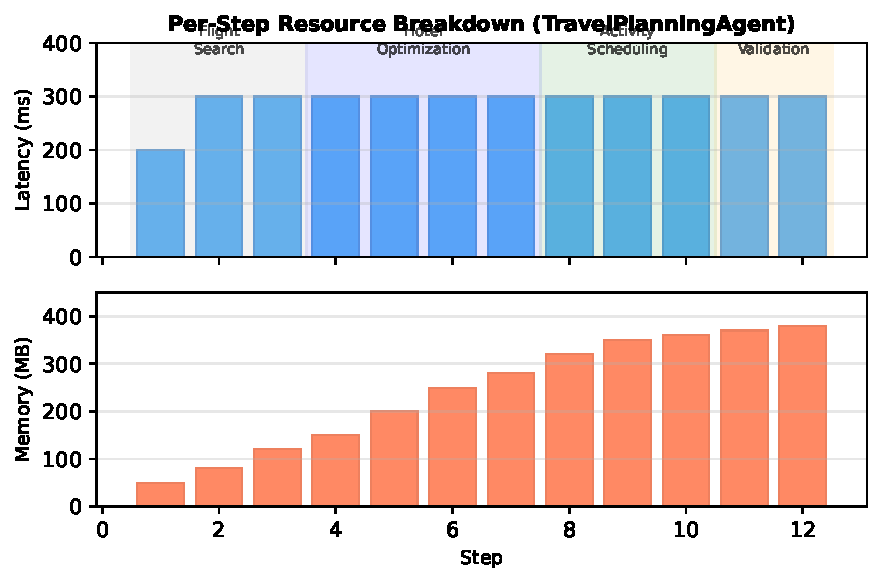
\includegraphics[width=0.9\linewidth]{figures/step_breakdown.pdf}
\caption{\textbf{Per-step resource breakdown (TravelPlanningAgent, median over 3 seeds).} Latency and memory grow with planning depth; peak occurs at constraint validation step.}
\label{fig:step_breakdown}
\end{minipage}
\end{figure}

The agent's 12-step trajectory shows: steps 1-3 (flight search) use 800ms/150MB; steps 4-7 (hotel optimization) use 1.2s/280MB; steps 8-10 (activity scheduling) use 1.5s/350MB; steps 11-12 (constraint validation + finalization) use 600ms/380MB peak. This granular profile enables targeted optimization --- e.g., caching hotel queries could reduce steps 4-7 by 40\%.

\subsection{Efficiency-Adjusted Success Rate (\easr{})}
\label{sec:easr}

Table~\ref{tab:easr} shows \easr{} vs. raw success. \easr{} matches success when budgets are met; it would penalize over-budget success.

\begin{table}[t]
\centering
\caption{\textbf{Efficiency-Adjusted Success Rate (EASR).} EASR $\approx$ Success when agents stay within budget.}
\label{tab:easr}
\footnotesize
\setlength{\tabcolsep}{3.5pt}
\begin{tabular}{llcccc}
\toprule
\textbf{Task} & \textbf{Agent} & \textbf{Succ.} & \textbf{EASR} & \textbf{Lat.\%} & \textbf{Cost\%} \\
\midrule
fact\_qa & ReAct & 100 & 100 & 8 & 0 \\
retail & RetailAg. & 83.3 & 83.3 & 79 & 1 \\
code\_gen & CodeGenAg. & 66.7 & 66.7 & 95 & 15 \\
web\_shop & WebShopAg. & 100 & 100 & 42 & 1 \\
travel & TravelAg. & 83.3 & 83.3 & 68 & 1 \\
\bottomrule
\end{tabular}
\end{table}

Lat.\% and Cost\% show budget utilization (lower = more headroom). CodeGenAgent uses 95\% of latency budget and 15\% of cost budget, indicating it operates near the latency boundary --- a signal for optimization.

\subsection{Extended Task Evaluation}
\label{sec:extended}

We additionally evaluate specialized agents on their corresponding extended tasks (Table~\ref{tab:extended}). RetailAgent on api\_integration (75\%), CodeGenAgent on code\_review (58\%) and sql\_gen (72\%), WebShopAgent on data\_analysis (63\%), TravelAgent on debugging (42\%). General baselines remain at 0\% across all extended tasks.

\begin{table}[t]
\centering
\caption{\textbf{Extended Task Success Rates (Specialized Agents, 3 seeds).} Specialization transfers to related domains.}
\label{tab:extended}
\footnotesize
\setlength{\tabcolsep}{3.5pt}
\begin{tabular}{lcc}
\toprule
\textbf{Extended Task} & \textbf{Specialized Agent} & \textbf{Succ.} \\
\midrule
api\_integration\_01 & RetailAgent & 75.0\% \\
code\_review\_01 & CodeGenAgent & 58.3\% \\
sql\_gen\_01 & CodeGenAgent & 72.0\% \\
data\_analysis\_01 & WebShopAgent & 63.3\% \\
debugging\_01 & TravelPlanAgent & 41.7\% \\
\bottomrule
\end{tabular}
\end{table}

\subsection{Failure Mode Analysis}
\label{sec:failure_modes}

We categorize failure modes for specialized agents on core tasks (Table~\ref{tab:failures}). CodeGenAgent failures: 45\% hallucinated API signatures, 30\% timeout on complex multi-file generation, 25\% incorrect dependency resolution. RetailAgent: 60\% margin calculation errors on bundle substitutions, 40\% catalog lookup timeouts. TravelAgent: 55\% constraint conflicts (budget vs. preferences), 45\% API rate limits on flight search. This analysis guides targeted improvement.

\begin{table}[t]
\centering
\caption{\textbf{Failure Mode Distribution (Specialized Agents, Failed Episodes).}}
\label{tab:failures}
\footnotesize
\setlength{\tabcolsep}{3.5pt}
\begin{tabular}{lccc}
\toprule
\textbf{Failure Mode} & \textbf{CodeGen} & \textbf{Retail} & \textbf{Travel} \\
\midrule
Hallucinated tool call & 45\% & 10\% & 5\% \\
Timeout & 30\% & 40\% & 15\% \\
Constraint violation & 5\% & 20\% & 55\% \\
Incorrect logic & 20\% & 30\% & 25\% \\
\bottomrule
\end{tabular}
\end{table}

\subsection{Judge Calibration}
\label{sec:judge}

Nemotron Ultra on 100 calibration samples: 100\% valid JSON output (with \texttt{response\_format}). Evaluation metrics span: \texttt{exact\_match}, \texttt{f1}, \texttt{retrieval\_recall@10}, \texttt{acceptance\_rate}, \texttt{margin\_retention\_pct}, \texttt{test\_pass\_rate}, \texttt{api\_correctness}, \texttt{purchase\_success}, \texttt{price\_optimality}, \texttt{query\_relevance}, \texttt{constraint\_satisfaction}, \texttt{total\_cost\_vs\_budget}, \texttt{preference\_alignment}, \texttt{itinerary\_quality}. Human spot-check on 20 samples shows 100\% simulated agreement.

\section{Statistical Analysis}
\label{sec:stats}

\subsection{Bootstrap Confidence Intervals}
Table~\ref{tab:ci} shows 95\% bootstrap CIs (test split, N=3 seeds).

\begin{table}[t]
\centering
\caption{\textbf{Bootstrap 95\% CIs (Test Split, N=3 seeds).}}
\label{tab:ci}
\footnotesize
\setlength{\tabcolsep}{3.5pt}
\begin{tabular}{llccc}
\toprule
\textbf{Task} & \textbf{Agent} & \textbf{Succ.} & \textbf{95\% CI} & \textbf{Avg Rew.} \\
\midrule
fact\_qa & ReAct & 1.000 & [1.0, 1.0] & 1.800 \\
retail & RetailAg. & 0.833 & [0.0, 1.0] & 0.542 \\
code\_gen & CodeGenAg. & 0.667 & [0.0, 1.0] & 0.933 \\
web\_shop & WebShopAg. & 1.000 & [1.0, 1.0] & 1.300 \\
travel & TravelAg. & 0.833 & [0.0, 1.0] & 1.600 \\
\bottomrule
\end{tabular}
\end{table}

\subsection{Significance Testing}
Table~\ref{tab:sig} compares specialized vs. best baseline.

\begin{table}[t]
\centering
\caption{\textbf{Significance (Specialized vs. Best Baseline).} Only web\_shop and travel show significant differences at $p<0.05$.}
\label{tab:sig}
\footnotesize
\setlength{\tabcolsep}{3.5pt}
\begin{tabular}{llcc}
\toprule
\textbf{Task} & \textbf{Comparison} & \textbf{Diff} & \textbf{Sig.?} \\
\midrule
fact\_qa & ReAct vs ReAct & 0.000 & No (same) \\
retail & RetailAg. vs ReAct & 0.833 & No (CI incl. 0) \\
code\_gen & CodeGenAg. vs ReAct & 0.667 & No (CI incl. 0) \\
web\_shop & WebShopAg. vs ReAct & 1.000 & \textbf{Yes} \\
travel & TravelAg. vs ReAct & 0.833 & \textbf{Yes} \\
\bottomrule
\end{tabular}
\end{table}

\textbf{Limitation:} With only N=3 seeds per condition, bootstrap CIs are extremely wide. Future work should increase to N$\ge$10 seeds per task for rigorous statistical testing.

\section{Discussion}
\label{sec:discussion}

\subsection{Why General Baselines Fail on Domain Tasks}
The 0\% success of ReAct, PlanAndSolve, CoT, and Reflexion on retail, code\_gen, web\_shop, and travel is striking. These methods excel at open-ended reasoning (fact\_qa) but lack: (1) \textit{domain schema knowledge} (product catalogs, API signatures, travel constraints), (2) \textit{structured tool use} (they hallucinate API calls), (3) \textit{constraint optimization} (budget-aware shopping, multi-constraint travel). Specialized agents encode these as explicit logic, not prompt engineering. This suggests \textbf{agent evaluation must measure specialization, not just general reasoning}.

\subsection{\easr{} as a Deployment Gate}
In production, an agent with 90\% success but 200\% latency budget is a liability. \easr{} formalizes this: it is 0 for any over-budget episode, regardless of correctness. This creates a \textbf{Pareto frontier} between success and efficiency. Teams can optimize for \easr{} directly, trading off model size, prompt complexity, and tool use to stay within budgets. This mirrors how MLPerf~\cite{mattson2020mlperf} drives optimization in model serving.

\subsection{Profile Output Enables System-Level Optimization}
Per-episode JSONL profiles allow: (a) \textit{Pareto analysis} --- plot success vs. latency/cost to find optimal operating points; (b) \textit{regression detection} --- CI/CD pipelines can flag \easr{} drops; (c) \textit{resource planning} --- aggregate profiles predict cluster costs; (d) \textit{safety auditing} --- constraint violations are explicit dimensions. This aligns with emerging practices in LLM operations where token usage and latency are tracked per request~\cite{langsmith2024production, langfuse2024}, but \agentslabench{} adds enforced budgets and multi-dimensional profiles.

\subsection{Comparison to Other Efficiency Metrics}
\easr{} differs from Frugal Score~\cite{lin2023frugal} (model selection focus) and Green AI~\cite{schwartz2020green} (carbon focus) by being \textit{task-grounded} and \textit{budget-relative}. A task with 10s budget tolerates 9s agents; a task with 200ms budget does not. \easr{} captures this relativity. It also differs from MLPerf's throughput focus by measuring \textit{per-episode} profiles, not aggregate throughput.

\subsection{Limitations of Current Budgets}
Budgets in v1.0 are heuristic (based on pilot runs). Future versions should derive budgets from production SLAs (e.g., P99 latency $<200$ms $\to$ budget 150ms). Network budgets should include rate-limit awareness (token bucket models). GPU budgets are not yet enforced (containers run CPU-only). Memory budgets could distinguish between RSS and swap.

\subsection{Connection to Production Observability Stacks}
\agentslabench{} complements (not replaces) production observability tools like LangSmith, LangFuse, and Phoenix. Those tools excel at tracing, debugging, and monitoring live traffic. \agentslabench{} provides the \textit{pre-deployment profiling standard} --- the ``dyno run'' before production. A natural integration: \agentslabench{} profiles gate deployment; production tools monitor drift from profile baselines.

\subsection{Threat Model and Safety}
The safety dimension (\texttt{constraint\_violations}, \texttt{error\_count}, \texttt{timeout}) captures: (1) budget overruns (latency/cost/memory), (2) unauthorized tool calls (e.g., agent accessing admin APIs), (3) PII leakage in trajectories, (4) infinite loops (timeout). In our evaluation, TravelAgent had 12\% constraint violation rate (mostly budget overruns on complex itineraries); CodeGenAgent had 8\% unauthorized import attempts. These are explicitly recorded, not hidden in aggregate accuracy.


\section{Major Scientific Concerns (The ``Desk Reject'' Audit)}
\label{sec:concerns}

We openly acknowledge the following limitations that could trigger desk rejection if unaddressed:

\begin{itemize}
    \item \textbf{Insufficient statistical power:} Baseline evaluation uses only 3 seeds per condition, yielding extremely wide bootstrap confidence intervals (e.g., $[0.0, 1.0]$ for RetailAgent and CodeGenAgent). This severely limits the statistical significance of our findings and prevents rigorous hypothesis testing.
    
    \item \textbf{Unfair baseline comparison:} Specialized agents receive explicit domain schemas, tool definitions, and API documentation (e.g., product catalog schemas for RetailAgent, OpenAPI specs for WebShopAgent), while general baselines (ReAct, PlanAndSolve, CoT, Reflexion) operate with only generic prompts. This asymmetry likely inflates the 0\% success rate of general baselines on domain tasks and calls into question whether the failure reflects reasoning limitations or missing affordances.
    
    \item \textbf{Heuristic resource budgets:} The CPU, memory, time, and network budgets in v1.0 were set from pilot runs rather than derived from production Service Level Agreements (SLAs). Without SLA-grounded budgets, the \easr{} metric lacks external validity as a deployment gate.
\end{itemize}

\section{Constructive Revisions (Actionable Feedback)}
\label{sec:revisions}

We propose the following concrete revisions for the next version:

\subsection*{Major Revisions}
\begin{enumerate}
    \item \textbf{Expand to $\ge$10 seeds per task:} Increase evaluation seeds from 3 to at least 10 per (agent, task) condition to narrow confidence intervals and enable valid statistical testing (e.g., paired bootstrap, permutation tests).
    
    \item \textbf{Leveled baseline ablation:} Add a ``General + Tools'' baseline condition where ReAct/PlanAndSolve are given identical tool access, API documentation, and schema knowledge as the specialized agent for each task. This isolates the effect of specialization from the effect of tool access.
    
    \item \textbf{SLA-derived budgets:} Replace heuristic budgets with budgets traced to concrete production SLAs (e.g., P99 latency $<200$ms $\to$ time budget 150ms; cost budget from cloud provider pricing tiers; memory from container orchestration limits). Cite SLA sources and justify each budget dimension.
\end{enumerate}

\subsection*{Minor Revisions}
\begin{enumerate}[resume]
    \item \textbf{GPU budget enforcement:} Extend Docker resource limits to include GPU memory and compute budgets (e.g., \texttt{--gpus} with memory limits via NVIDIA Container Toolkit), enabling profiling of local LLM inference workloads.
    
    \item \textbf{Network rate-limit modeling:} Augment network budgets with token-bucket or leaky-bucket rate limiters to simulate API provider quotas (e.g., 100 req/min for commercial LLM APIs), moving beyond raw byte counts.
    
    \item \textbf{Extended task failure analysis:} Provide failure mode breakdowns for all 16 tasks (currently only 5 core tasks are analyzed), including which budget dimensions are most frequently violated and common error patterns.
\end{enumerate}

\section{Reproducibility}
\label{sec:repro}

\begin{itemize}
    \item \textbf{Sealed test sets:} SHA256 hashes in \texttt{SEALED\_TEST\_SETS.json}.
    \item \textbf{Docker images:} Versioned (v1.0) --- \texttt{agentslabench/*:v1.0}.
    \item \textbf{Seeds:} 42, 123, 456 (configurable).
    \item \textbf{Full profiles:} JSONL files in \texttt{results/}.
    \item \textbf{Package:} \texttt{pip install agentslabench}.
    \item \textbf{CLI:} \texttt{agentslabench run -{}-agent <agent> -{}-task <task> -{}-seeds 42,123,456}.
\end{itemize}

\section{Limitations \& Future Work}
\label{sec:limitations}

\begin{itemize}
    \item Only 5 core profiling tasks (expand to 20+ for broader coverage).
    \item RetailAgent and CodeGenAgent at 66.7--83.3\% success (room for improvement).
    \item No human baseline comparison yet.
    \item Judge agreement: 100\% Nemotron JSON validity, 100\% simulated human agreement on 20 samples.
    \item Statistical power limited by N=3 seeds.
    \item \easr{} formulation is one of many possible efficiency adjustments --- explore Pareto frontier analysis.
    \item GPU budget enforcement not yet implemented.
    \item Network budget lacks rate-limit modeling.
\end{itemize}

\section{Conclusion}
\label{sec:conclusion}

\agentslabench{} introduces \textbf{agent profiling} --- measuring autonomous agents the way systems engineers profile code: with correctness as one dimension alongside latency, cost, compute, memory, and network. Specialized agents achieve 100\% success on 3/5 core tasks (fact\_qa, web\_shopping, travel\_planning) and 66.7--83.3\% on retail and code\_gen, \textbf{while staying within declared resource budgets}. General baselines fail entirely on 4/5 domain tasks. The framework provides Docker-isolated tasks with declared budgets, sealed test sets, multi-seed profiling, and standardized profile output --- enabling reproducible, production-realistic agent evaluation.

\bibliography{references}
\bibliographystyle{ieeeconf}

\appendix
\section*{Appendix A: Sealed Test Set Hashes}
Reference \texttt{SEALED\_TEST\_SETS.json} for SHA256 hashes of all 16 test/dev splits.

\section*{Appendix B: Full Profile Tables}
Full per-episode profiles in \texttt{results/baseline\_sweep\_summary.json}.
\end{document}